% Created 2023-11-20 Mon 23:25
% Intended LaTeX compiler: pdflatex
\documentclass[11pt]{article}
\usepackage[utf8]{inputenc}
\usepackage[T1]{fontenc}
\usepackage{graphicx}
\usepackage{longtable}
\usepackage{wrapfig}
\usepackage{rotating}
\usepackage[normalem]{ulem}
\usepackage{amsmath}
\usepackage{amssymb}
\usepackage{capt-of}
\usepackage{hyperref}
\author{谢树强}
\date{\today}
\title{}
\hypersetup{
 pdfauthor={谢树强},
 pdftitle={},
 pdfkeywords={},
 pdfsubject={},
 pdfcreator={Emacs 29.1 (Org mode 9.6.6)}, 
 pdflang={English}}
\begin{document}

\tableofcontents

\section{1.1 什么是因特网}
\label{sec:orgba7f4c7}

\begin{figure}[htbp]
\centering
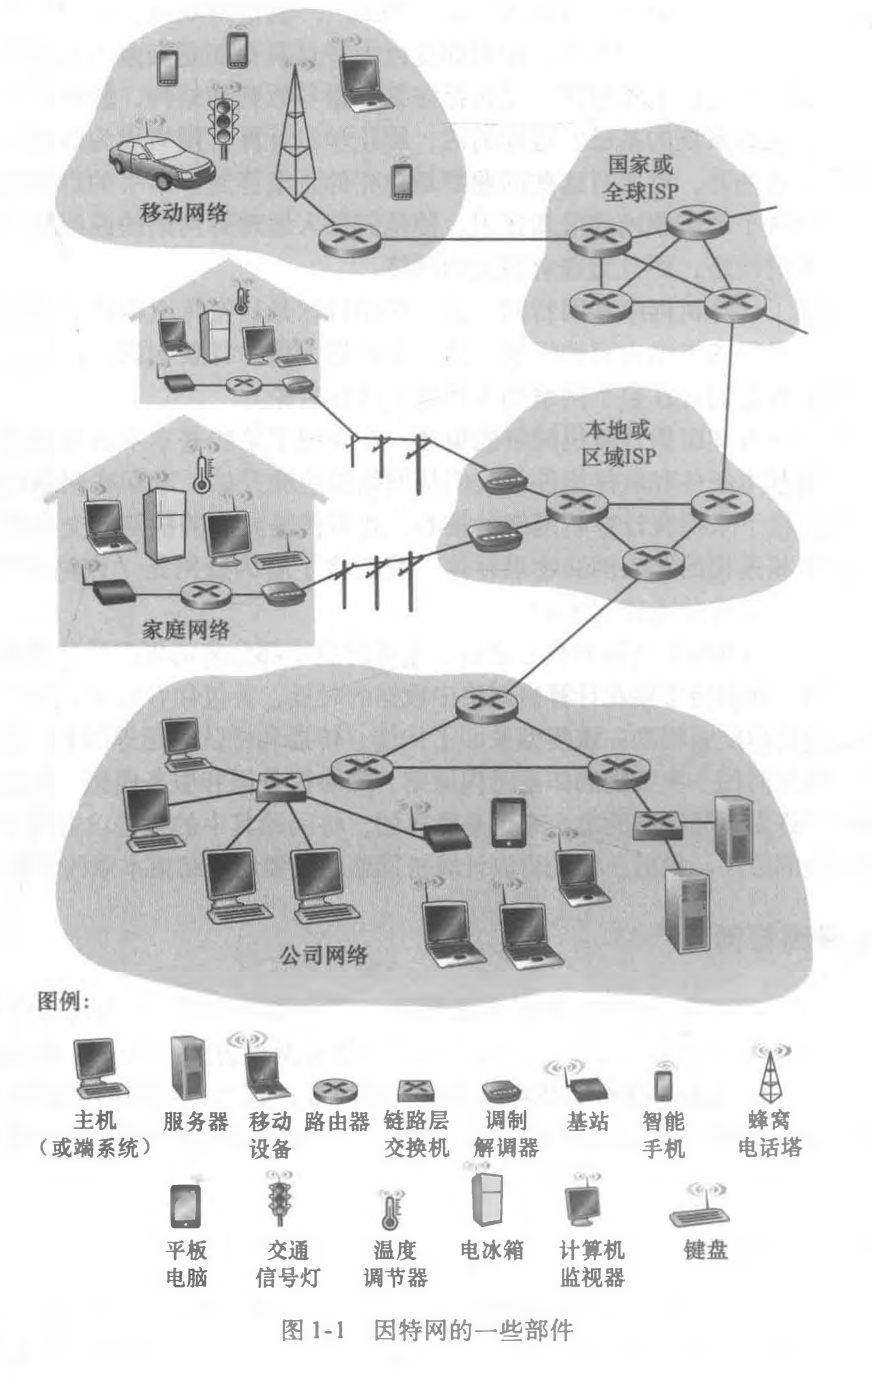
\includegraphics[width=.9\linewidth]{imag/Snipaste_2023-11-19_12-29-46.png}
\caption{因特网的组成部分(图)}
\end{figure}

\subsection{1.1.1 具体构成}
\label{sec:org998b900}

\subsubsection{名词解释}
\label{sec:org49979cb}
\begin{enumerate}
\item 端系统/主机
\end{enumerate}
\begin{verbatim}
构成因特网的初始部分,包括手机,电脑,服务器,电视游戏机,家用电器,手表、眼睛、汽车、运输控制系统等;上面的图片有所显示;
\end{verbatim}

\texttt{主机通过 *通信链路* 和 *分组交换机* 连接到一起}

\begin{enumerate}
\item 通信链路
\begin{verbatim}
信号传输的媒介包括:同轴电缆、铜线、光纤和无线电频谱。
\end{verbatim}
\item 传输速率
\begin{verbatim}
以比特/秒(bit/s或bps)度量。
\end{verbatim}
\item 分组
\begin{verbatim}
一台端系统向另一台端系统发送数据时,发送端数据将数据分段,并为每段加上首部字节,这样形成的信息包称为分组(也就是封包)
分组交换是相对于电路交换来说的,就是传输之前不需要确定通信路径.
\end{verbatim}
\item 分组交换机
可以实现分组通信的交换机;现在最流行的是两种。 \textbf{路由器}  和 \textbf{链路层} 交换机
\item 路径(route/path)
\begin{verbatim}
从发送端系统到接收端系统,一个数据包所经历的一系列通信链路和分组交换机称为经过该网络的路径;
\end{verbatim}
\item 因特网服务提供商(Internet Service Provider,ISP)
\begin{verbatim}
端系统通过ISP接入因特网,每个ISP自身就是由一个多台分组交换机和多段通信链路组成的网络;包括各种类型如下
\end{verbatim}

\begin{itemize}
\item 本地电缆或电话公司的住宅区ISP
\item 公司ISP
\item 大学ISP
\item 机场、咖啡店、旅馆和其他公共场所提供的WiFi接入的ISP
\item 手机和其他移动设备的移动接入的蜂窝数据ISP
\end{itemize}
\end{enumerate}
\begin{quote}
ISP 提供多种类型的因特网连接,包括但不限于:
宽带接入: 提供常见的家庭和企业宽带服务,例如数字订阅线路(DSL)、光纤(Fiber)、电缆互联网(Cable Internet)等。
移动网络: 提供移动数据服务,允许用户通过移动电话、移动热点或移动数据设备连接因特网,包括 4G 和 5G 网络。
企业服务: 提供专门面向企业客户的服务,如专线连接、托管服务、云服务等。
\end{quote}

\begin{enumerate}
\item 协议
\begin{verbatim}
端系统、分组交换机和因特网的一些其他部件都要运行一些协议,这些协议控制因特网中信息的接收和发送;
\end{verbatim}

\begin{itemize}
\item \texttt{TCP(Transmission Control Protocol,传输控制协议)}
\item \texttt{IP(Internet Protocol,网际协议)}
\end{itemize}
\end{enumerate}











\subsection{1.1.2 服务描述}
\label{sec:org70de470}
\textbf{从为应用程序提供服务的基础设施} 的角度来描述因特网;这就是 \texttt{套接字} 接口,该接口规定了运行在一个端系统的程序请求因特网
基础设施向运行另一个端系统上的特定目的地程序交付数据方式;就是不同程序通过这个接口可以将数据发送到互联网当中,无论我们使用
什么样的语言,java,C,pathon都没有影响;

\subsection{1.1.3 什么是协议}
\label{sec:org3ec6f61}
协议(protocol)就是交互双方共同遵从的一套规范,在这个规范下双方才能够“理解”对方的问题,并给出回答,回答的内容也能够
使提问方理解;
\texttt{协议(protocol)定义了在两个或多个通信实体之间交换的报文的格式和顺序,以及报文发送和/或接收一条报文或其他事件所采取的动作}


\section{1.2 网络边缘}
\label{sec:orgcfdd8cb}

网络边缘指的就是指日常使用的计算机,智能手机和其他设备;其实就是互联网的最先部分;

\subsection{1.2.1 接入网}
\label{sec:org408bef3}
将端系统物理连接到其边缘路由器的网络。边缘路由器是端系统到其他任何远程端系统的路径上的第一台路由器;

\begin{enumerate}
\item \texttt{家庭接入:DSL、电缆、FTTH、拨号和卫星}
数字用户线(Digital Subscriber Line,DSL)和电缆是最常用的两种方式
\textbf{DSL是一种接入的技术,可以使用电话线作为载体}
\begin{figure}[htbp]
\centering
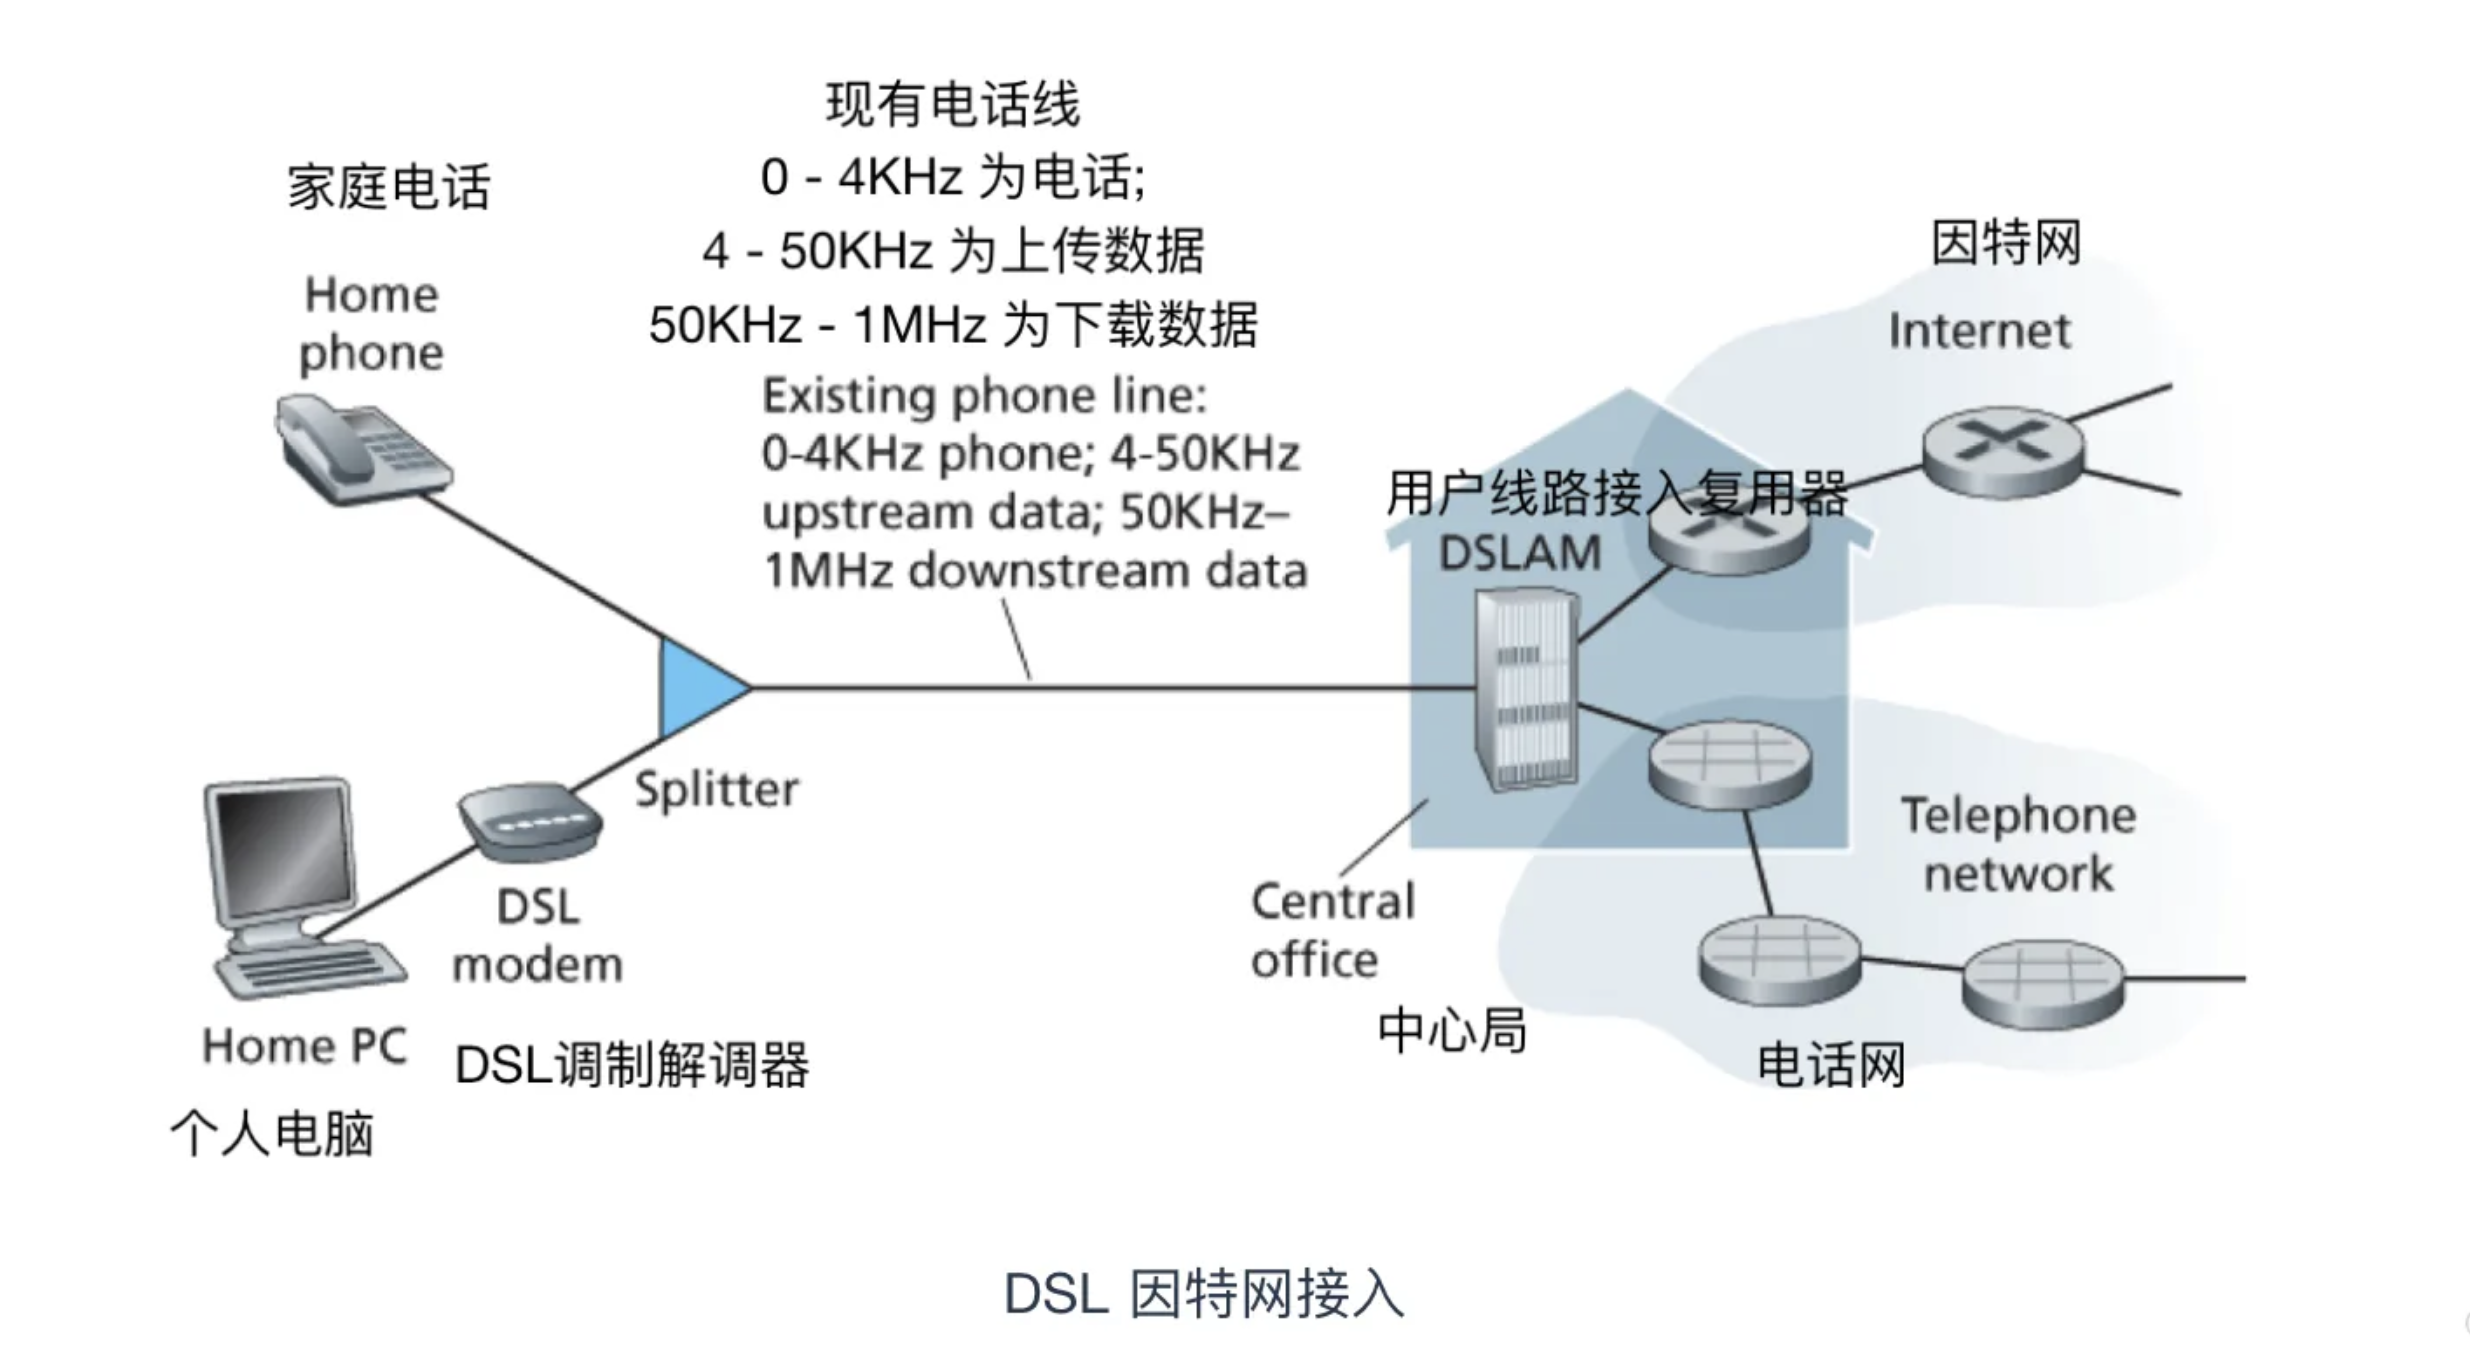
\includegraphics[width=.9\linewidth]{imag/Snipaste_2023-11-19_23-58-23.png}
\caption{DSL因特网接入(图)}
\end{figure}

\begin{figure}[htbp]
\centering
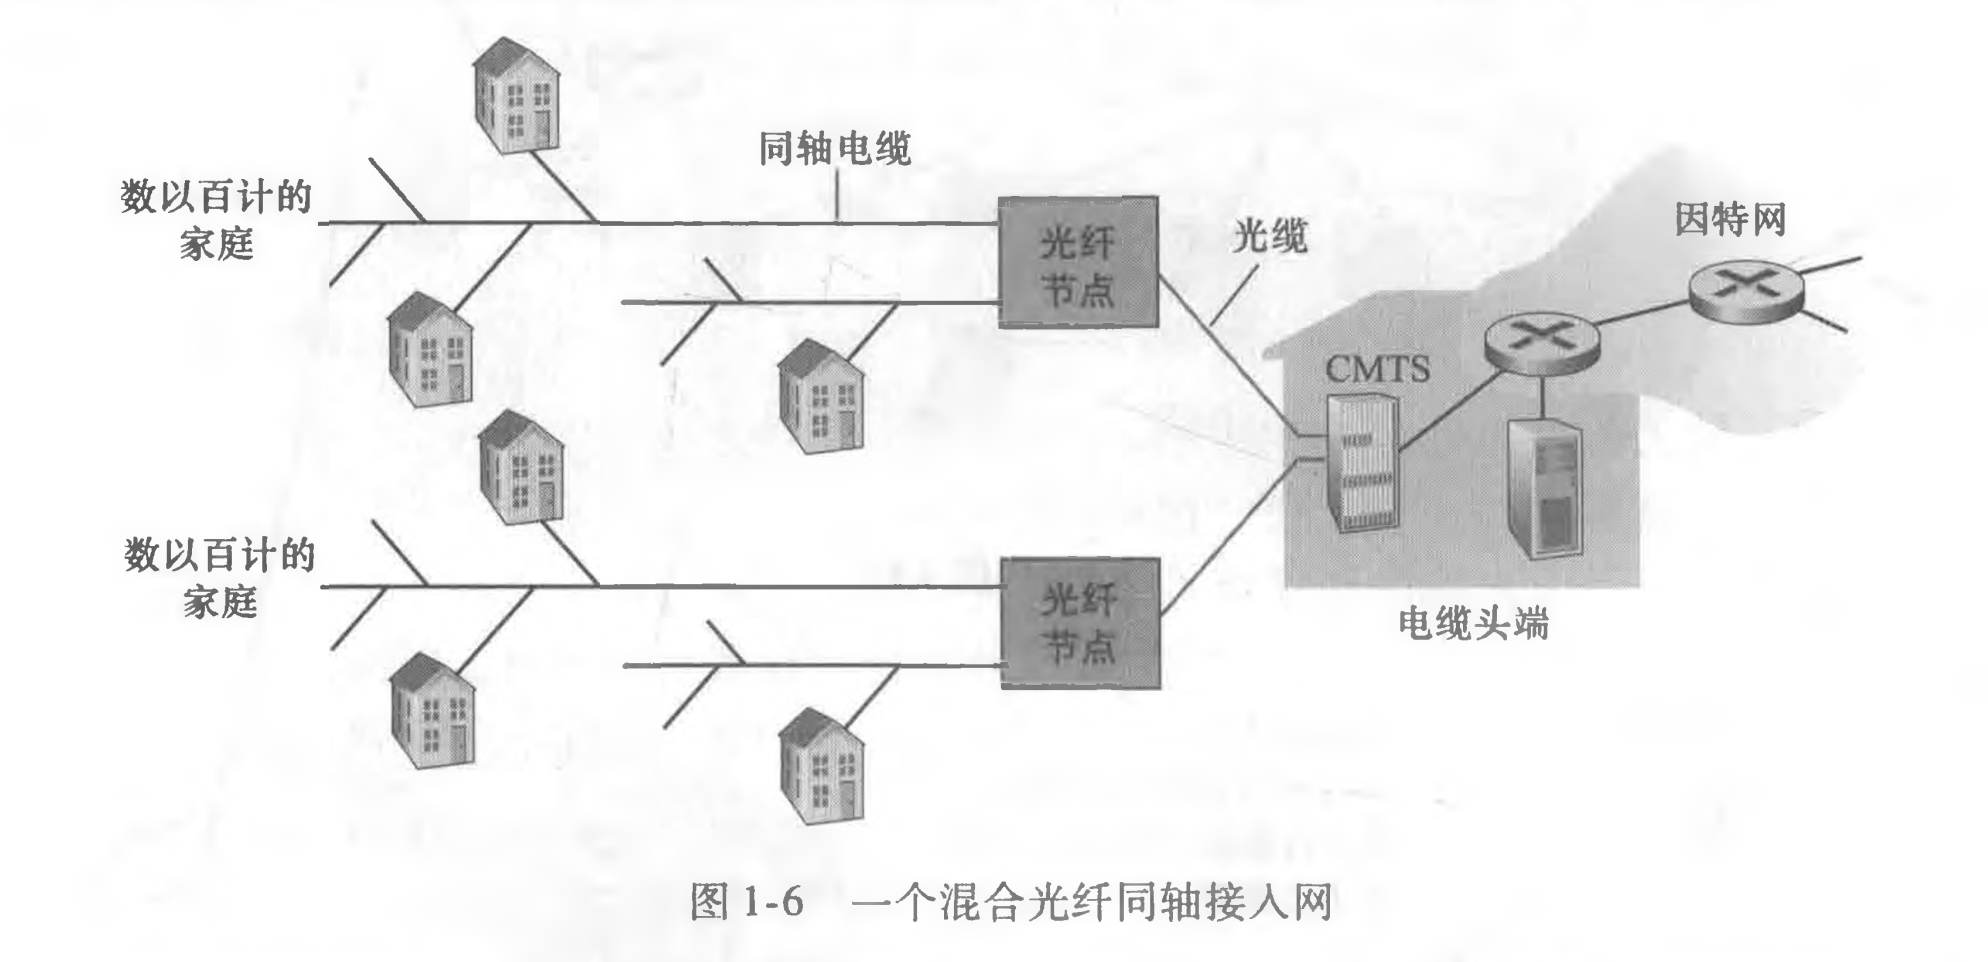
\includegraphics[width=.9\linewidth]{imag/Snipaste_2023-11-20_20-31-47.png}
\caption{电缆光纤同轴(图)}
\end{figure}

\begin{figure}[htbp]
\centering
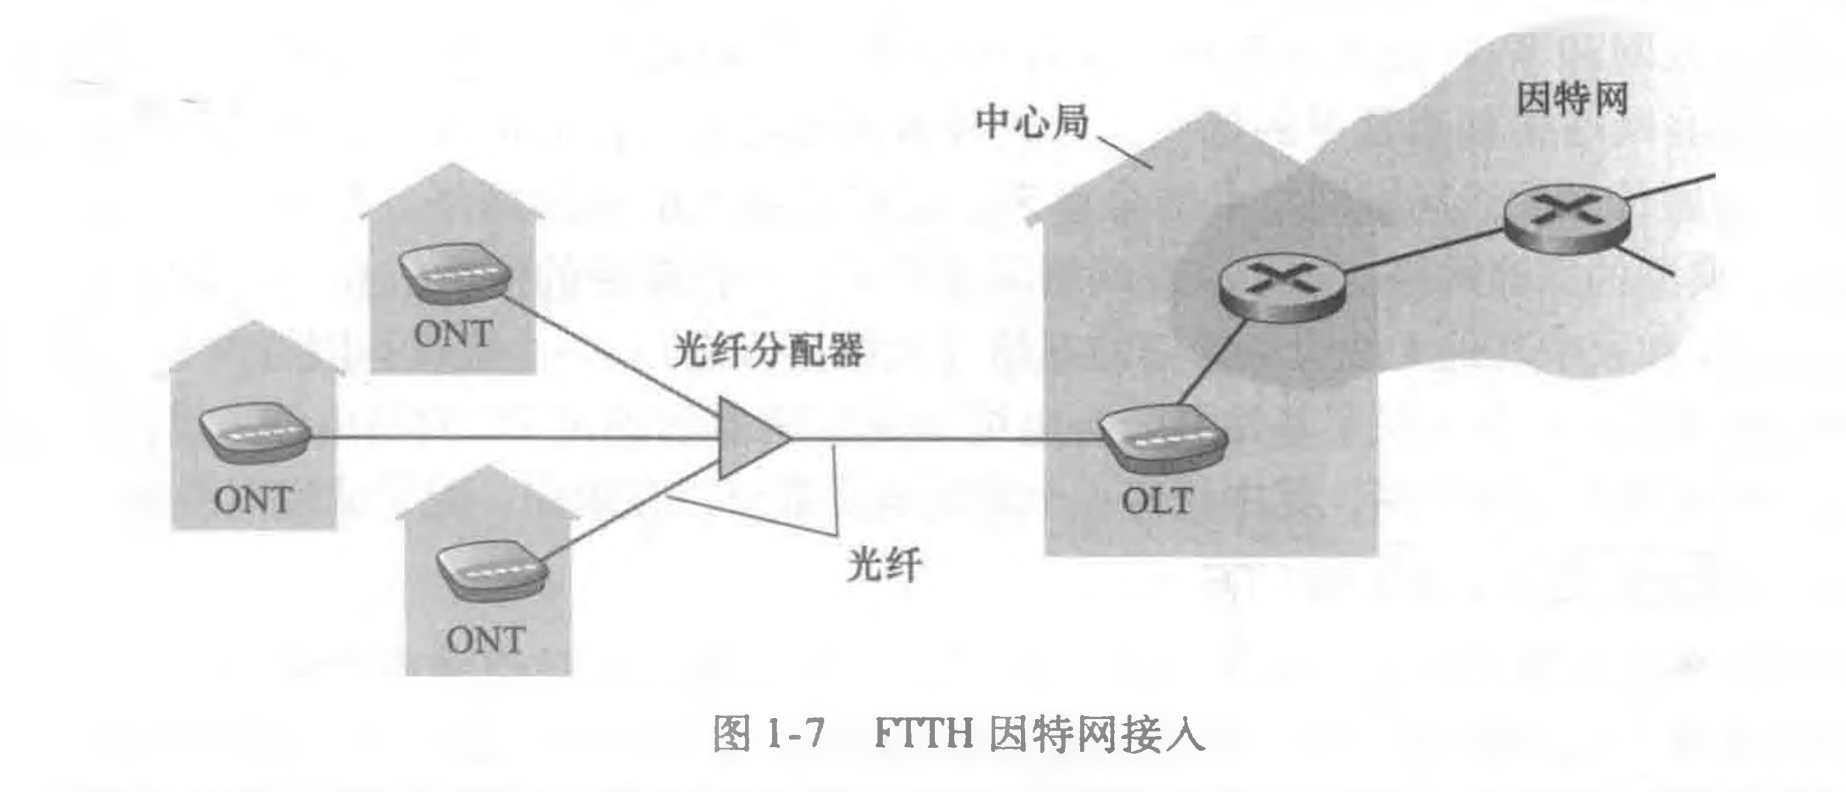
\includegraphics[width=.9\linewidth]{imag/Snipaste_2023-11-20_20-44-33.png}
\caption{FTTH光纤接入(图)}
\end{figure}

\item \texttt{企业(和家庭)接入:以太网和Wi-Fi}
以太网就是通过网线直接接入,后者舍弃了网线使用Wi-Fi接收信号;
\begin{figure}[htbp]
\centering
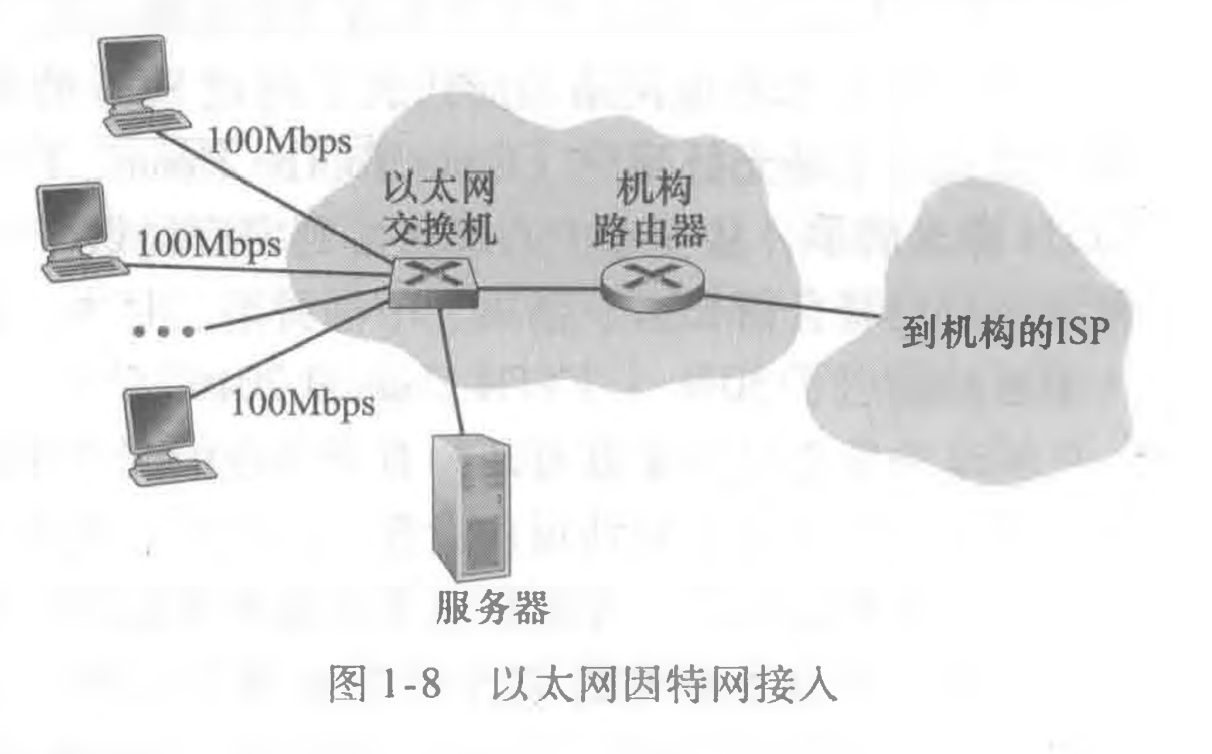
\includegraphics[width=.9\linewidth]{imag/Snipaste_2023-11-20_20-55-20.png}
\caption{以太网接入(图)}
\end{figure}

\begin{figure}[htbp]
\centering
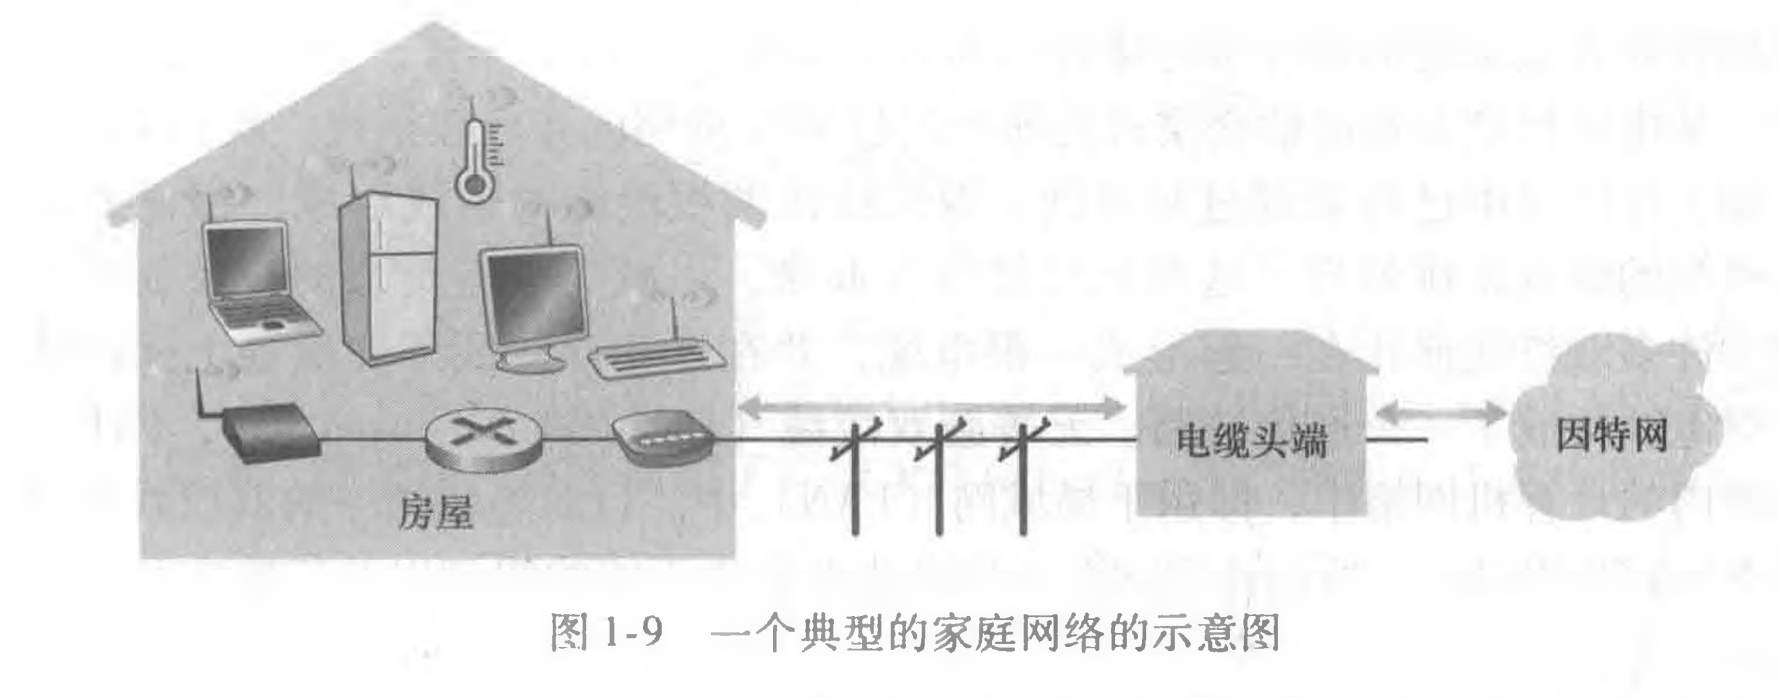
\includegraphics[width=.9\linewidth]{imag/Snipaste_2023-11-20_20-59-20.png}
\caption{wifi接入(图)}
\end{figure}

\item \texttt{广域无线接入:3G和LTE}
基站和蜂窝网络,就是现在手机使用的;不过4G也已经普及了,5G投资有点失败。
\end{enumerate}













\subsection{1.2.2 物理媒体}
\label{sec:orgac0e9f2}
指网络信号传输的介质,可以分为两种类型, \texttt{引导型}  \texttt{非引导型}
引导型电波沿着媒体前行,如光缆、双绞铜线、或同轴电缆
非引导型电波沿着空气或外太空传播,例如无线局域网或数字卫星频道
\begin{enumerate}
\item 双绞铜线
\begin{verbatim}
也叫双绞线,就是我们平时说的网线,每两根绞合在一起;DSL技术配合双绞线可以使用户以数十Mbps的速率接入因特网。
\end{verbatim}
\item 同轴电缆
\begin{verbatim}
一般作为电视信号线,有段时间国家一直推广的有线电视。
\end{verbatim}
\item 光纤
\begin{verbatim}
光纤线一般作为宽带接入线,现在已经普及。
\end{verbatim}
\item 陆地无线电信道
\begin{verbatim}
一般分为三类,一类距离很短,1-2米,如无线耳机,键盘等设备;无线LAN技术,也就是现在的Wi-Fi;第三类运行很广,跨越\\
\end{verbatim}

数万米,例如蜂窝接入技术使用了广域无线电信道;
\item 卫星无线电信道
\end{enumerate}


\section{1.3 网络核心}
\label{sec:orgde4f677}
\begin{quote}
即由互联因特网端系统的分组交换机和链路构成的网状网络;
\end{quote}

\subsection{1.3.1 分组交换}
\label{sec:org789189c}
分组交换是指对于端系统要传输的信号,一般会分成多个包进行传输,这个传输称为分组;分组有两个特点:
\begin{enumerate}
\item 存储转发传输
\begin{verbatim}
指一个分组(包)必须全部到达路由器才会进行转发,不是一进入路由器就开始转发,以包为单位;
\end{verbatim}
\item 排队时延和分组丢失
\begin{verbatim}
每个路由器都有工作能力的上限,如果前面的转发没有结束就会进入等待,排队满了就会发生包丢失现象,没法接收新的包;
\end{verbatim}
\item 转发表和路由协议
\begin{verbatim}
路由器中有一个转发表,告诉路由器应该把包转发到哪个路由器上面;
\end{verbatim}

\textbf{路由器识别包的路径根据IP地址,不是识别整个地址,而是识别其中的一部分确定下一个路由器,
然后下一个识别别的部分,经过多个识别转发到正确的地址} ;
\end{enumerate}
\end{document}